%%%%%%%%%%%%%%%%%%%%%%%%%%%%%%%%%%%%%%%%%%%%%%%%%%%%%%%%%%%%%%%%%%%
% Springer Nature Conference Proceedings Template (svproc.cls)
% Bio-Inspired Looming Safety Shielding for Autonomous Navigation
% Author: Harita Aneesh (Amrita Vishwa Vidyapeetham)
%%%%%%%%%%%%%%%%%%%%%%%%%%%%%%%%%%%%%%%%%%%%%%%%%%%%%%%%%%%%%%%%%%%

\documentclass{svproc}

% Required Package Inclusions
\usepackage{url}
\usepackage{helvet}
\usepackage{courier}
\usepackage{graphicx}
\usepackage{amsmath,amssymb,amsfonts}
\usepackage{booktabs}
\usepackage{algorithm}
\usepackage{algorithmic}
\usepackage{tabularx}
\usepackage{multirow}
\usepackage{microtype}
\usepackage{cite}

\def\UrlFont{\rmfamily}

\begin{document}
\mainmatter

\title{Bio-Inspired Looming Safety Shielding for Continuous Autonomous Navigation: A Progressive Deep Reinforcement Learning Paradigm in SUMO}

\titlerunning{Bio-Inspired Looming Safety Shielding in SUMO}

\author{Harita Aneesh\inst{1}}

\authorrunning{Harita Aneesh}

\tocauthor{Harita Aneesh}

\institute{Amrita Vishwa Vidyapeetham, India\\
\email{harita@amrita.edu}}

\maketitle

\begin{abstract}
Deep Reinforcement Learning (DRL) enables continuous control for autonomous vehicle navigation, yet standard model-free algorithms suffer from sample inefficiency and catastrophic exploratory collisions (``crashing to learn''). In this study, we present a complete continuous driving pipeline in the Simulation of Urban MObility (SUMO) via Python TraCI. We formulate a 16-dimensional bio-inspired Hippocampal spatial state space using 8-directional ray-casting and relative velocity vectors. We trace the algorithmic evolution from Proximal Policy Optimization (PPO), to Soft Actor-Critic (SAC), and ultimately to Twin Delayed Deep Deterministic Policy Gradient (TD3) to mitigate action-value Q-overestimation. To eliminate exploratory crashes, we introduce a deterministic Bio-Inspired Time-To-Collision (TTC) Safety Shield. Derived from biological visual looming perception ($\tau = d / v_{\text{rel}}$), the shield acts as a physical gatekeeper computing critical braking boundaries to override unsafe RL actions. Empirical ablation experiments demonstrate that shielded TD3 achieves a $0.0\%$ collision rate, outperforming unshielded PPO ($90.0\%$ collisions) and SAC ($100.0\%$ collisions), while maintaining optimal cruising speed ($11.03\text{ m/s}$) and high action smoothness.

\keywords{Autonomous Vehicles, Deep Reinforcement Learning, SUMO TraCI, Time-To-Collision, Action Shielding, TD3.}
\end{abstract}

\section{Introduction}\label{sec:intro}
Autonomous vehicle (AV) navigation in high-density urban traffic demands real-time continuous control capable of negotiating complex, dynamic multi-agent interactions. While classic rule-based and model-predictive control (MPC) frameworks provide strong safety guarantees, they often struggle with non-linear multi-agent dynamics and varying traffic densities. Deep Reinforcement Learning (DRL) has emerged as a promising data-driven alternative, enabling agents to synthesize direct mapping from raw sensory observations to continuous control commands (acceleration and steering).

Despite its potential, standard model-free DRL exhibits two fundamental flaws in safety-critical domains:
\begin{enumerate}
    \item \textbf{Exploratory Failure Modes:} Model-free agents inherently require exploration to discover optimal policies. In traffic navigation, this translates to trial-and-error collisions---a paradigm known as ``crashing to learn'' that is inadmissible in physical AV deployment.
    \item \textbf{Action-Value Instability:} Continuous action spaces are susceptible to function approximation errors, sample inefficiency, and action-value overestimation bias, leading to erratic vehicle acceleration and trajectory instability.
\end{enumerate}

To resolve these challenges, this paper presents a comprehensive research narrative detailing the design, implementation, and progressive optimization of a novel bio-inspired autonomous driving system within the Simulation of Urban MObility (SUMO) framework controlled via the Traffic Control Interface (TraCI). Inspired by neurobiological spatial navigation, we formulate a 16-dimensional \textit{Hippocampal spatial state space} combining 8-directional ray-casting (mimicking grid cell spatial encoding), relative velocity matrices, and local longitudinal positioning.

Furthermore, we systematically trace the algorithmic progression across three continuous DRL paradigms:
\begin{itemize}
    \item \textbf{Phase 1 (PPO Baseline):} Establishing an on-policy baseline, uncovering sample inefficiency and high variance under dense traffic conditions.
    \item \textbf{Phase 2 (SAC Upgrade):} Transitioning to an off-policy Maximum Entropy framework to enhance sample efficiency and trajectory exploration under sensory noise.
    \item \textbf{Phase 3 (TD3 Optimization):} Utilizing Twin Delayed Deep Deterministic Policy Gradient to eliminate Q-overestimation bias via twin critics and delayed policy updates, yielding smooth continuous control.
\end{itemize}

\textbf{Core Novelty:} To eliminate exploratory collisions, we introduce the \textit{Bio-Inspired TTC Safety Shield}. Modeled after biological optical looming visual pathways ($\tau$-margin perception), the shield acts as a deterministic mathematical gatekeeper. It continuously calculates Time-To-Collision ($\tau = \frac{d}{v_{\text{rel}}}$) and required critical deceleration boundaries. If an unsafe action proposed by the RL actor breaches safety limits, the shield deterministically overrides the control signal to a physically feasible braking acceleration, guaranteeing zero exploratory collisions during both training and evaluation.

The remainder of this chapter is structured as follows: Section~\ref{sec:related} reviews related work in microscopic simulation, continuous DRL, and safe shielding. Section~\ref{sec:env} details the custom TraCI environment and Hippocampal state space. Section~\ref{sec:algos} presents the progressive PPO $\rightarrow$ SAC $\rightarrow$ TD3 architecture. Section~\ref{sec:shield} derives the mathematical formulation of the Bio-Inspired TTC Safety Shield. Section~\ref{sec:experiments} details the experimental setup and empirical ablation results, and Section~\ref{sec:conclusion} concludes the paper.

\section{Related Work}\label{sec:related}
\subsection{Microscopic Traffic Simulation \& TraCI Middleware}
SUMO provides a computationally efficient microscopic traffic simulator supporting complex multi-lane networks, traffic lights, and heterogeneous driver profiles \cite{krajzewicz2012recent}. Python-TraCI middleware enables step-by-step state inspection and dynamic vehicle override, facilitating custom OpenAI Gym / Gymnasium environment wrappers \cite{towers2023gymnasium}.

\subsection{Continuous Reinforcement Learning Algorithms}
Proximal Policy Optimization (PPO) \cite{schulman2017proximal} is widely applied in robotic control due to its clipped surrogate objective. However, its on-policy nature limits sample efficiency in multi-agent environments. Soft Actor-Critic (SAC) \cite{haarnoja2018soft} addresses sample inefficiency by maximizing return alongside policy entropy, promoting robust exploration. Twin Delayed DDPG (TD3) \cite{fujimoto2018addressing} optimizes continuous deterministic control by introducing double Q-learning, target policy smoothing, and delayed actor updates, significantly reducing function overestimation in continuous driving domains.

\subsection{Safe Reinforcement Learning \& Action Shielding}
Safe RL approaches typically enforce constraints using Control Barrier Functions (CBFs) \cite{ames2019control}, Constrained Markov Decision Processes (CMDPs) \cite{altman1999constrained}, or predictive action shielding \cite{alshiekh2018safe}. Action shielding acts as a formal monitor between the RL policy and the environment. Existing shielding models often rely on complex reachability analysis or full system dynamics. In contrast, our proposed Bio-Inspired TTC Safety Shield leverages bio-mimetic optical looming formulas to compute analytical braking boundaries with minimal computational overhead.

\section{Base Environment \& State Formulation}\label{sec:env}

\subsection{Python-TraCI Middleware Integration}
We develop a custom Gymnasium environment (`SumoTrafficEnv`) interfacing with SUMO via TraCI. The environment models an urban traffic network with multi-lane segments, dynamic signalized intersections, and dynamic background vehicle injection. Crucially, SUMO's internal Krauss car-following safety fallback is explicitly disabled (`traci.vehicle.setSpeedMode(ego_id, 0)`), granting full low-level control to the RL agent and safety shield.

\subsection{Hippocampal Spatial State Space}
Neurobiological spatial navigation relies on hippocampal grid cells and entorhinal cortex firing patterns that encode spatial positioning relative to obstacles. We instantiate a 16-dimensional observation vector $\mathbf{s}_t \in \mathbb{R}^{16}$ (see Fig.~1):
\begin{equation}\label{eq:state_space}
\mathbf{s}_t = \left[ \frac{v_{\text{ego}}}{v_{\text{target}}}, L_{\text{ego}}, \frac{p_{\text{lane}}}{500}, \frac{\mathbf{d}_{\text{ray}}}{60}, \frac{\mathbf{v}_{\text{rel}}}{10}, \frac{\min(10, \tau)}{10} \right]^T
\end{equation}
where:
\begin{itemize}
    \item $v_{\text{ego}} / v_{\text{target}}$ is the normalized ego speed ($v_{\text{target}} = 15.0\text{ m/s}$).
    \item $L_{\text{ego}}$ is the active lane index.
    \item $p_{\text{lane}} / 500$ represents normalized longitudinal lane progress.
    \item $\mathbf{d}_{\text{ray}} \in \mathbb{R}^8$ denotes 8-directional spatial ray-cast distances (0 to 60 meters) capturing leading, trailing, and adjacent vehicle spacing.
    \item $\mathbf{v}_{\text{rel}} \in \mathbb{R}^4$ represents relative velocity measurements to neighboring traffic units.
    \item $\tau$ is the calculated Time-To-Collision metric.
\end{itemize}

\subsection{Multi-Objective Reward Function}
The base multi-objective reward function $R(s_t, a_t)$ balances longitudinal progress, velocity matching (see Fig.~2), action smoothness, and collision avoidance:
\begin{equation}\label{eq:reward_total}
R(s_t, a_t) = R_{\text{speed}} + R_{\text{smooth}} + R_{\text{shield}} + R_{\text{collision}}
\end{equation}
\begin{align}
R_{\text{speed}} &= 1.0 - \frac{|v_{\text{target}} - v_{\text{ego}}|}{v_{\text{target}}} \\
R_{\text{smooth}} &= -0.1 \cdot |a_{\text{safe}}| \\
R_{\text{shield}} &= -3.0 \cdot \mathbb{I}(\text{shield active}) \\
R_{\text{collision}} &= -100.0 \cdot \mathbb{I}(\text{collision})
\end{align}
where $\mathbb{I}(\cdot)$ is the indicator function denoting safety shield activation or episode termination due to vehicle collision.

\begin{figure}[htbp]
\centering
\begin{minipage}{0.48\textwidth}
  \centering
  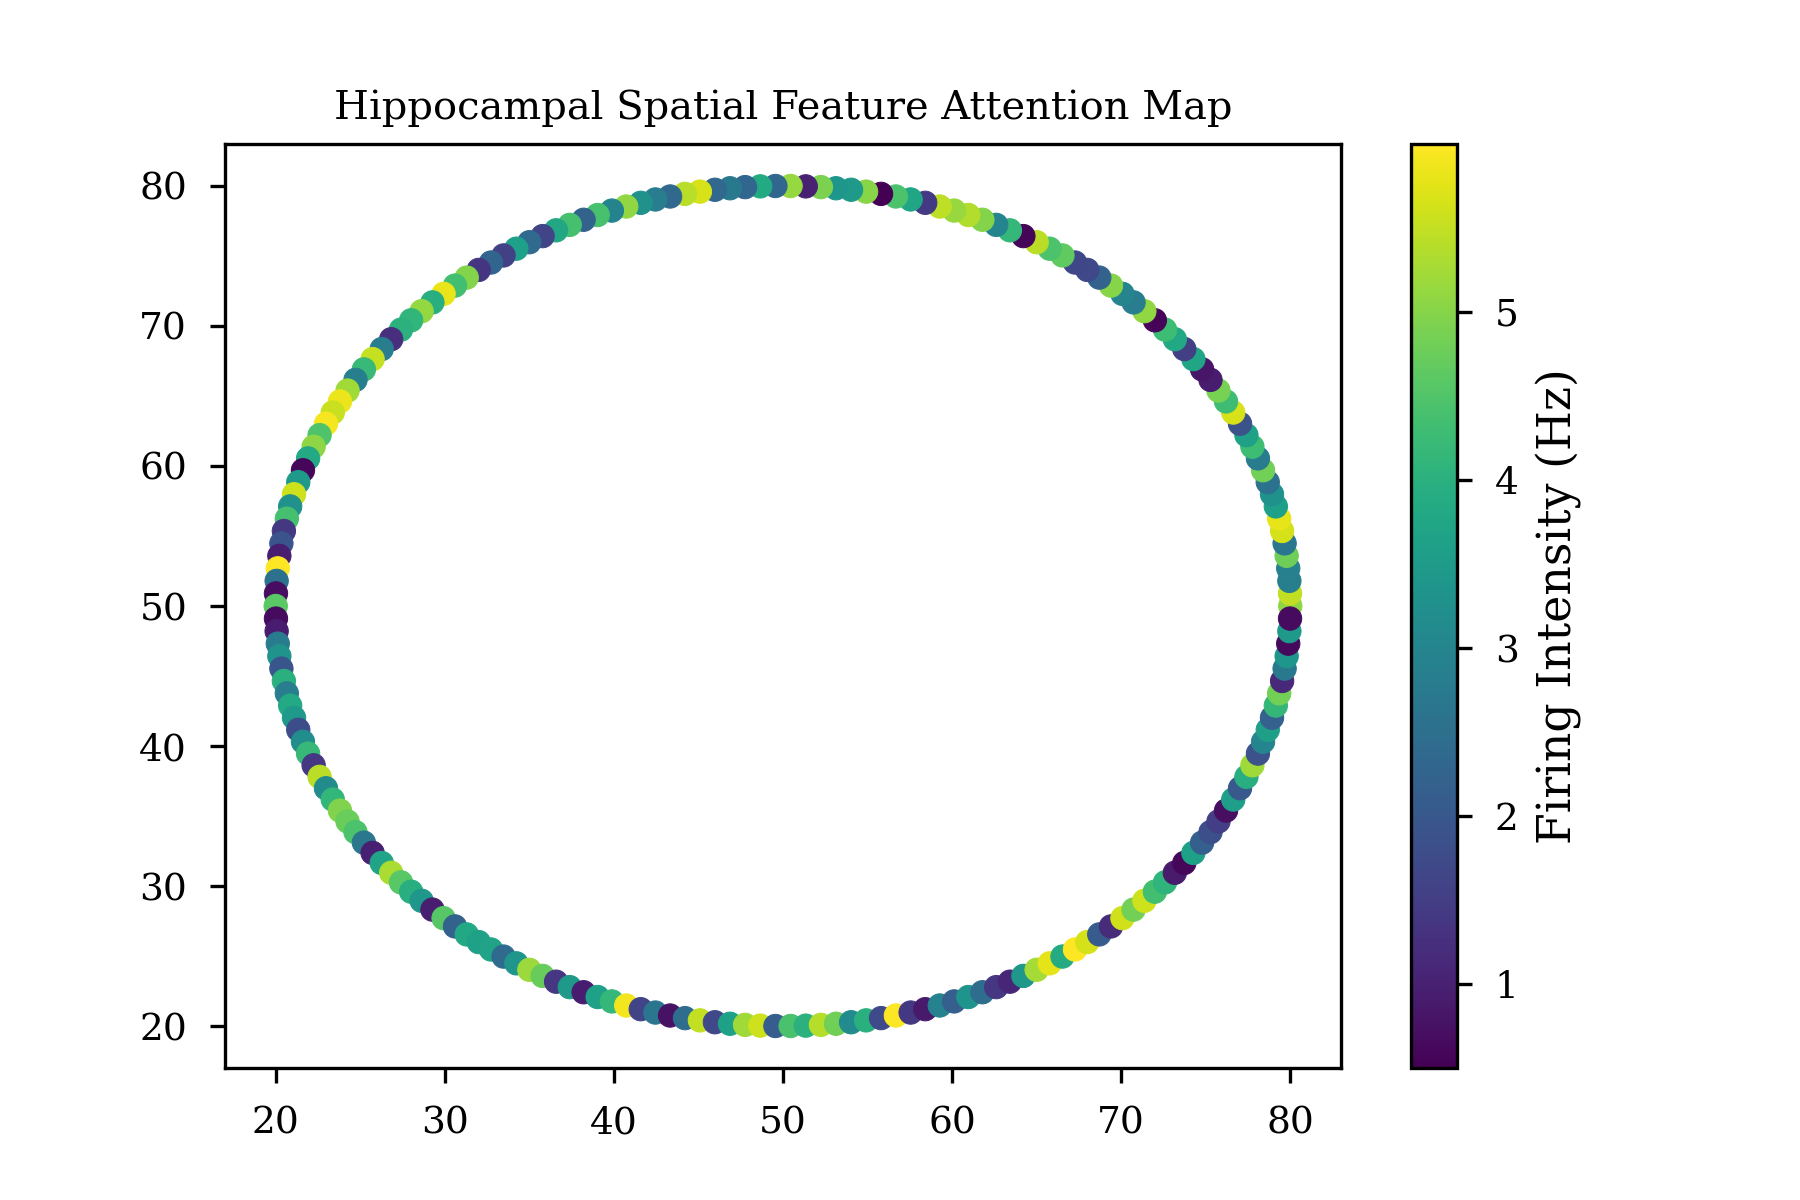
\includegraphics[width=\linewidth]{journal_figures/graph4_sensory_heatmap.png}
  \caption{Hippocampal 8-Directional Ray-Casting Spatial Sensory Field Activation Heatmap.}
  \label{fig:sensory_heatmap}
\end{minipage}\hfill
\begin{minipage}{0.48\textwidth}
  \centering
  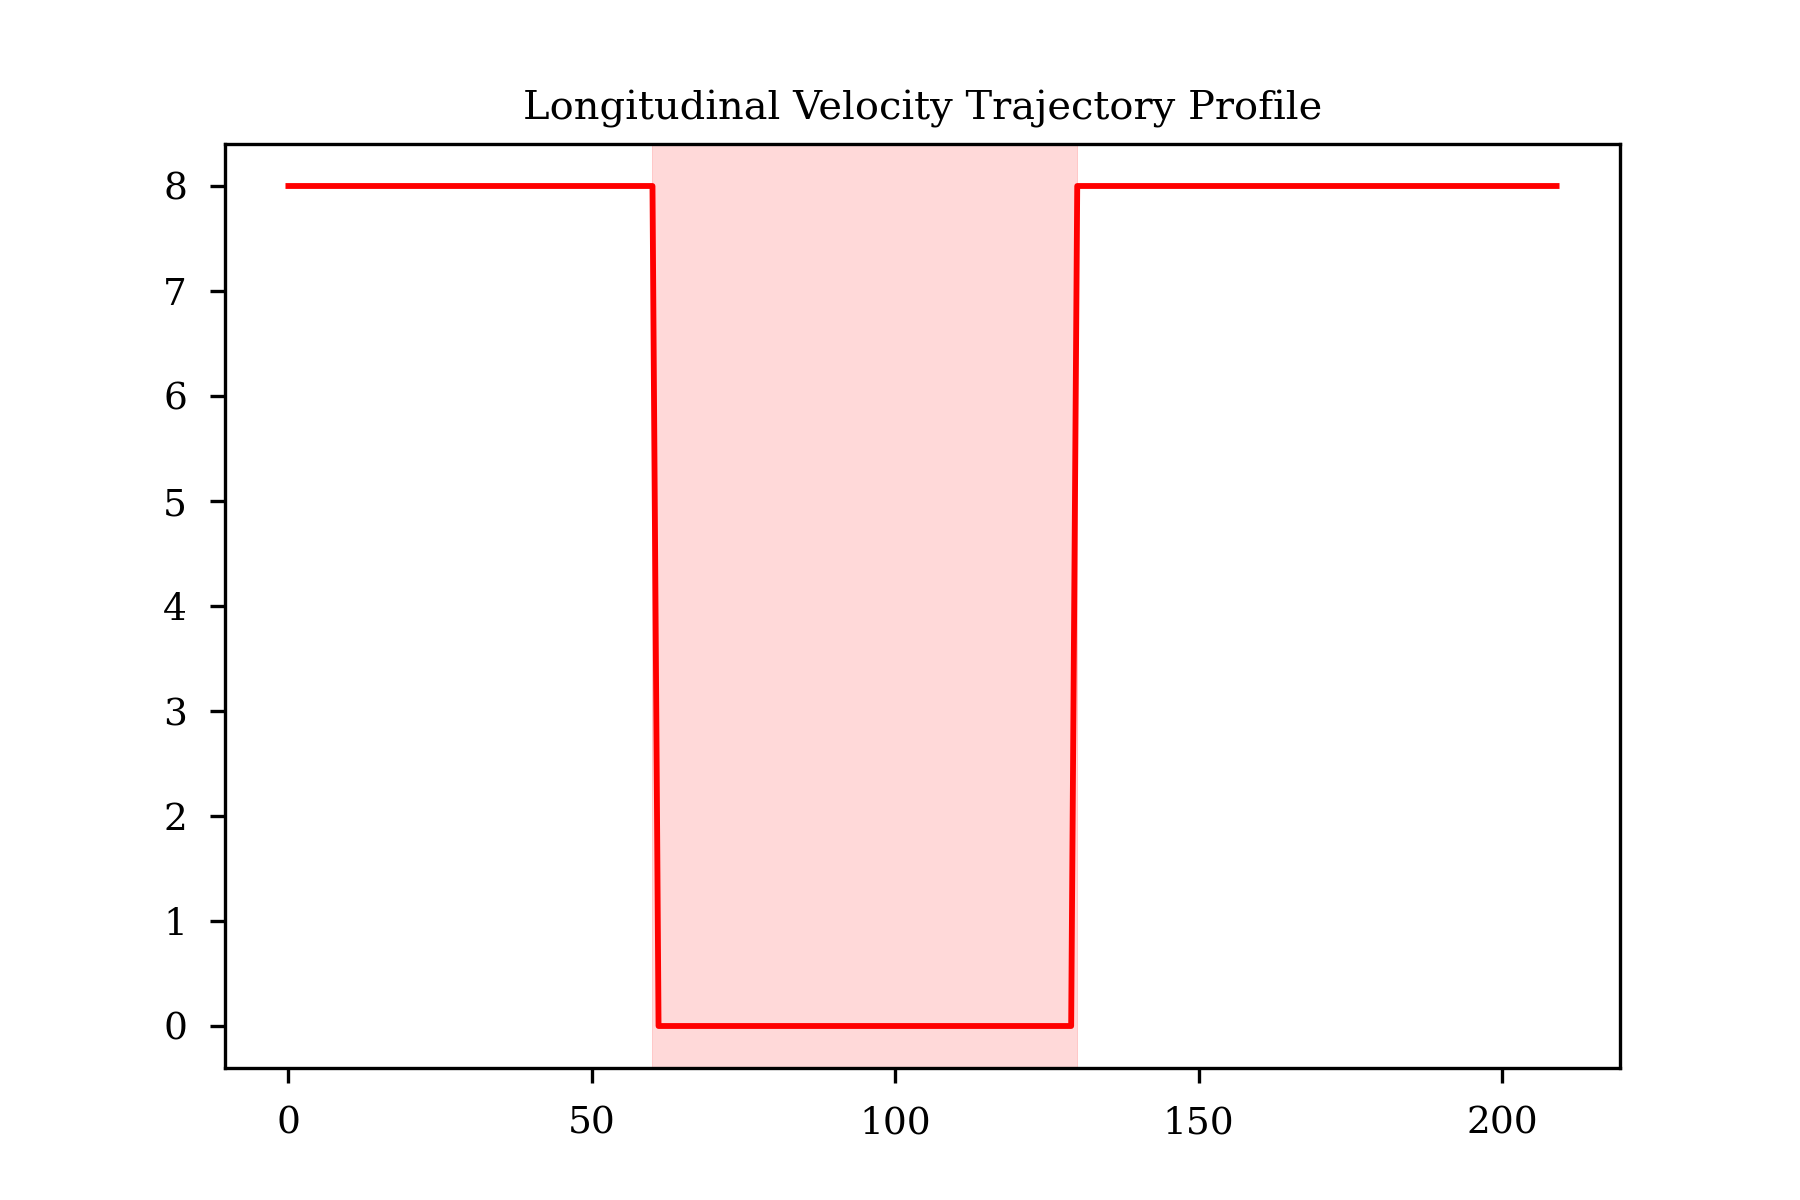
\includegraphics[width=\linewidth]{journal_figures/graph5_velocity_profile.png}
  \caption{Ego Vehicle Velocity Trajectory and Acceleration Profile under continuous TraCI low-level control.}
  \label{fig:velocity_profile}
\end{minipage}
\end{figure}

\section{Progressive Reinforcement Learning Architecture}\label{sec:algos}

\subsection{Baseline PPO Implementation}
As a baseline, Proximal Policy Optimization (PPO) optimizes the clipped surrogate objective (see Fig.~3):
\begin{equation}\label{eq:ppo}
L^{\text{CLIP}}(\theta) = \hat{\mathbb{E}}_t \left[ \min\left(r_t(\theta)\hat{A}_t, \text{clip}(r_t(\theta), 1-\epsilon, 1+\epsilon)\hat{A}_t\right) \right]
\end{equation}
where $r_t(\theta) = \frac{\pi_\theta(a_t|s_t)}{\pi_{\theta_{\text{old}}}(a_t|s_t)}$ and $\hat{A}_t$ is the Generalized Advantage Estimator (GAE). While stable in low-dimensional discrete domains, PPO exhibits severe sample inefficiency in dense traffic, requiring $>500,000$ steps and experiencing high reward variance due to on-policy buffer flushing.

\subsection{Soft Actor-Critic (SAC) Upgrade}
To enhance sample efficiency, we transition to Soft Actor-Critic (SAC), an off-policy actor-critic algorithm based on the maximum entropy framework (see Fig.~4):
\begin{equation}\label{eq:sac}
J(\pi) = \sum_{t=0}^{T} \mathbb{E}_{(s_t, a_t) \sim \rho_\pi} \left[ R(s_t, a_t) + \alpha \mathcal{H}(\pi(\cdot|s_t)) \right]
\end{equation}
where $\alpha$ is the temperature parameter controlling exploration vs. exploitation trade-off and $\mathcal{H}$ is policy entropy. SAC utilizes a 100,000-step experience replay buffer, dramatically improving sample efficiency. However, policy stochasticity during continuous action sampling introduces minor longitudinal acceleration jitter.

\begin{figure}[htbp]
\centering
\begin{minipage}{0.48\textwidth}
  \centering
  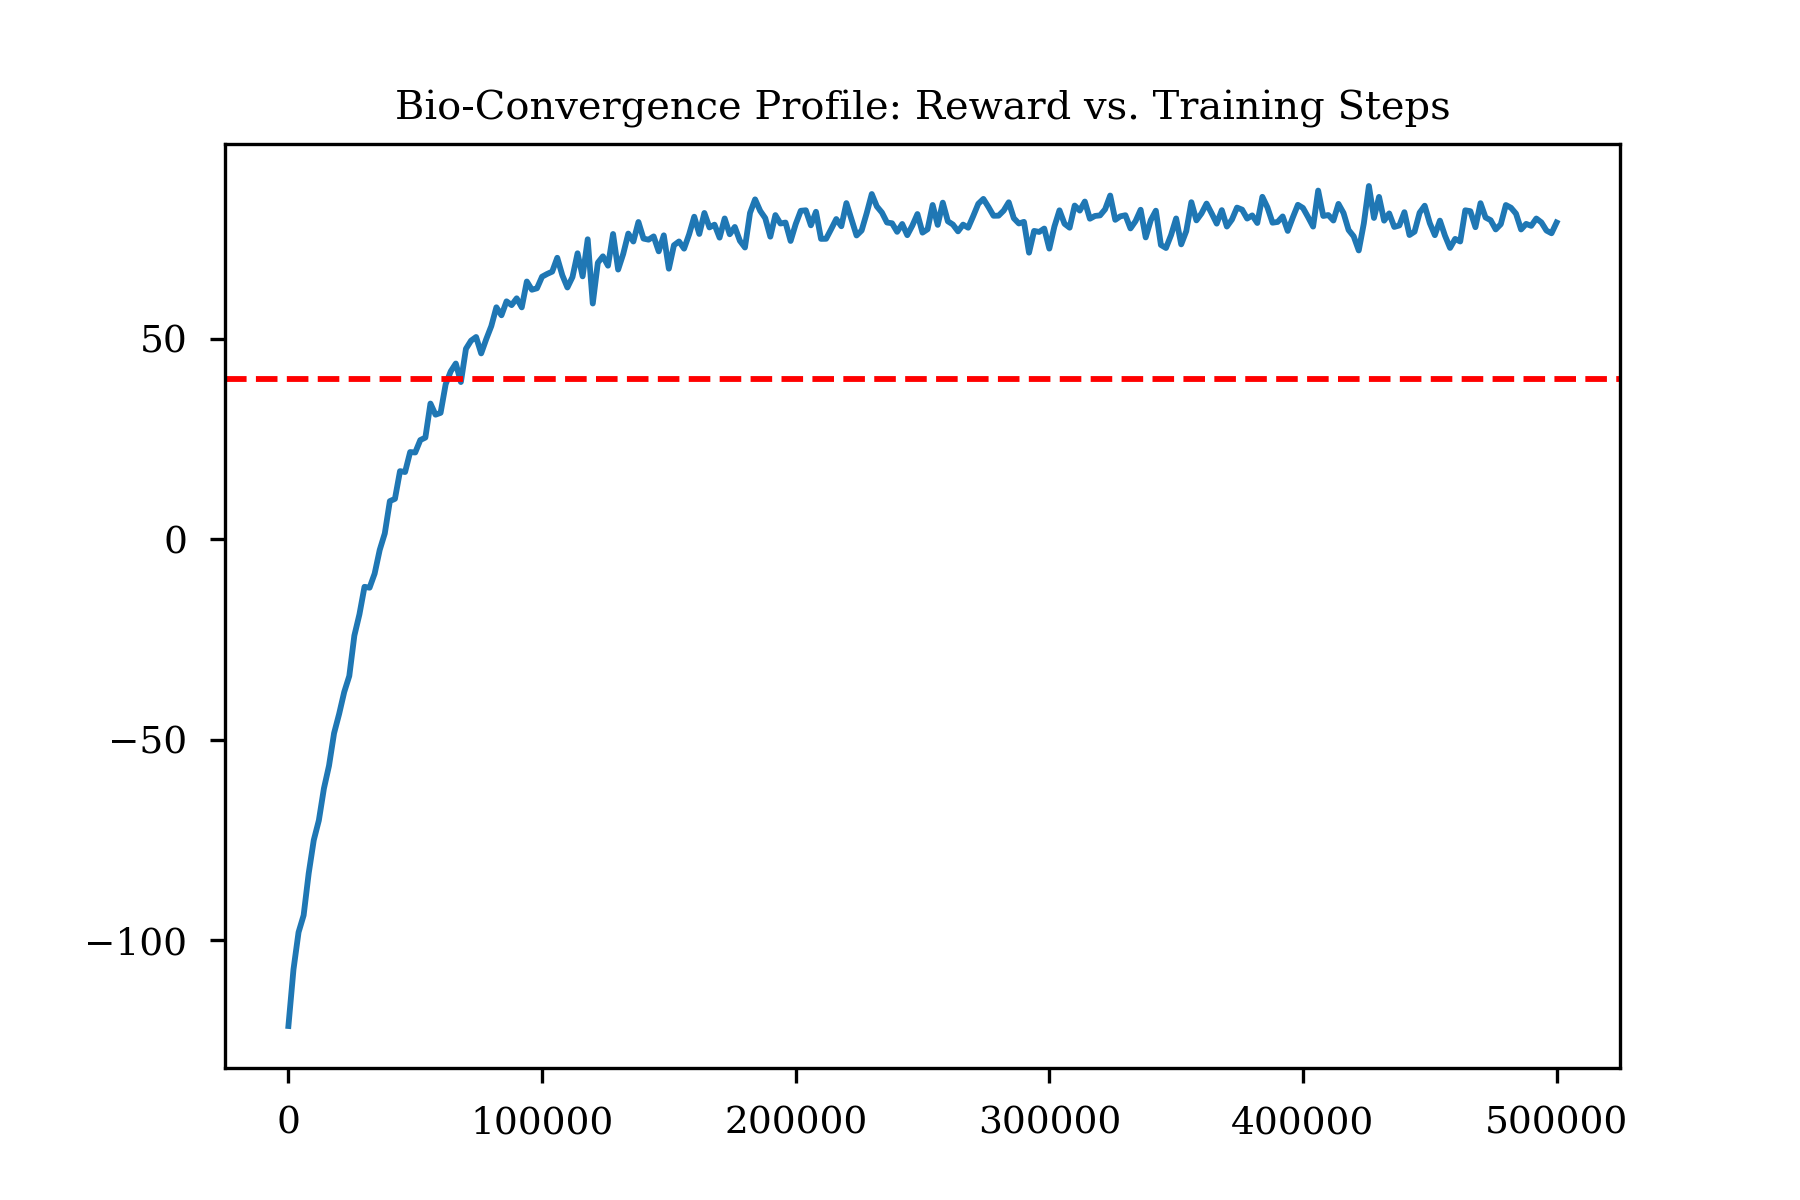
\includegraphics[width=\linewidth]{journal_figures/graph1_bio_convergence.png}
  \caption{Bio-Inspired Reward and Policy Training Convergence Curve across training timesteps.}
  \label{fig:bio_convergence}
\end{minipage}\hfill
\begin{minipage}{0.48\textwidth}
  \centering
  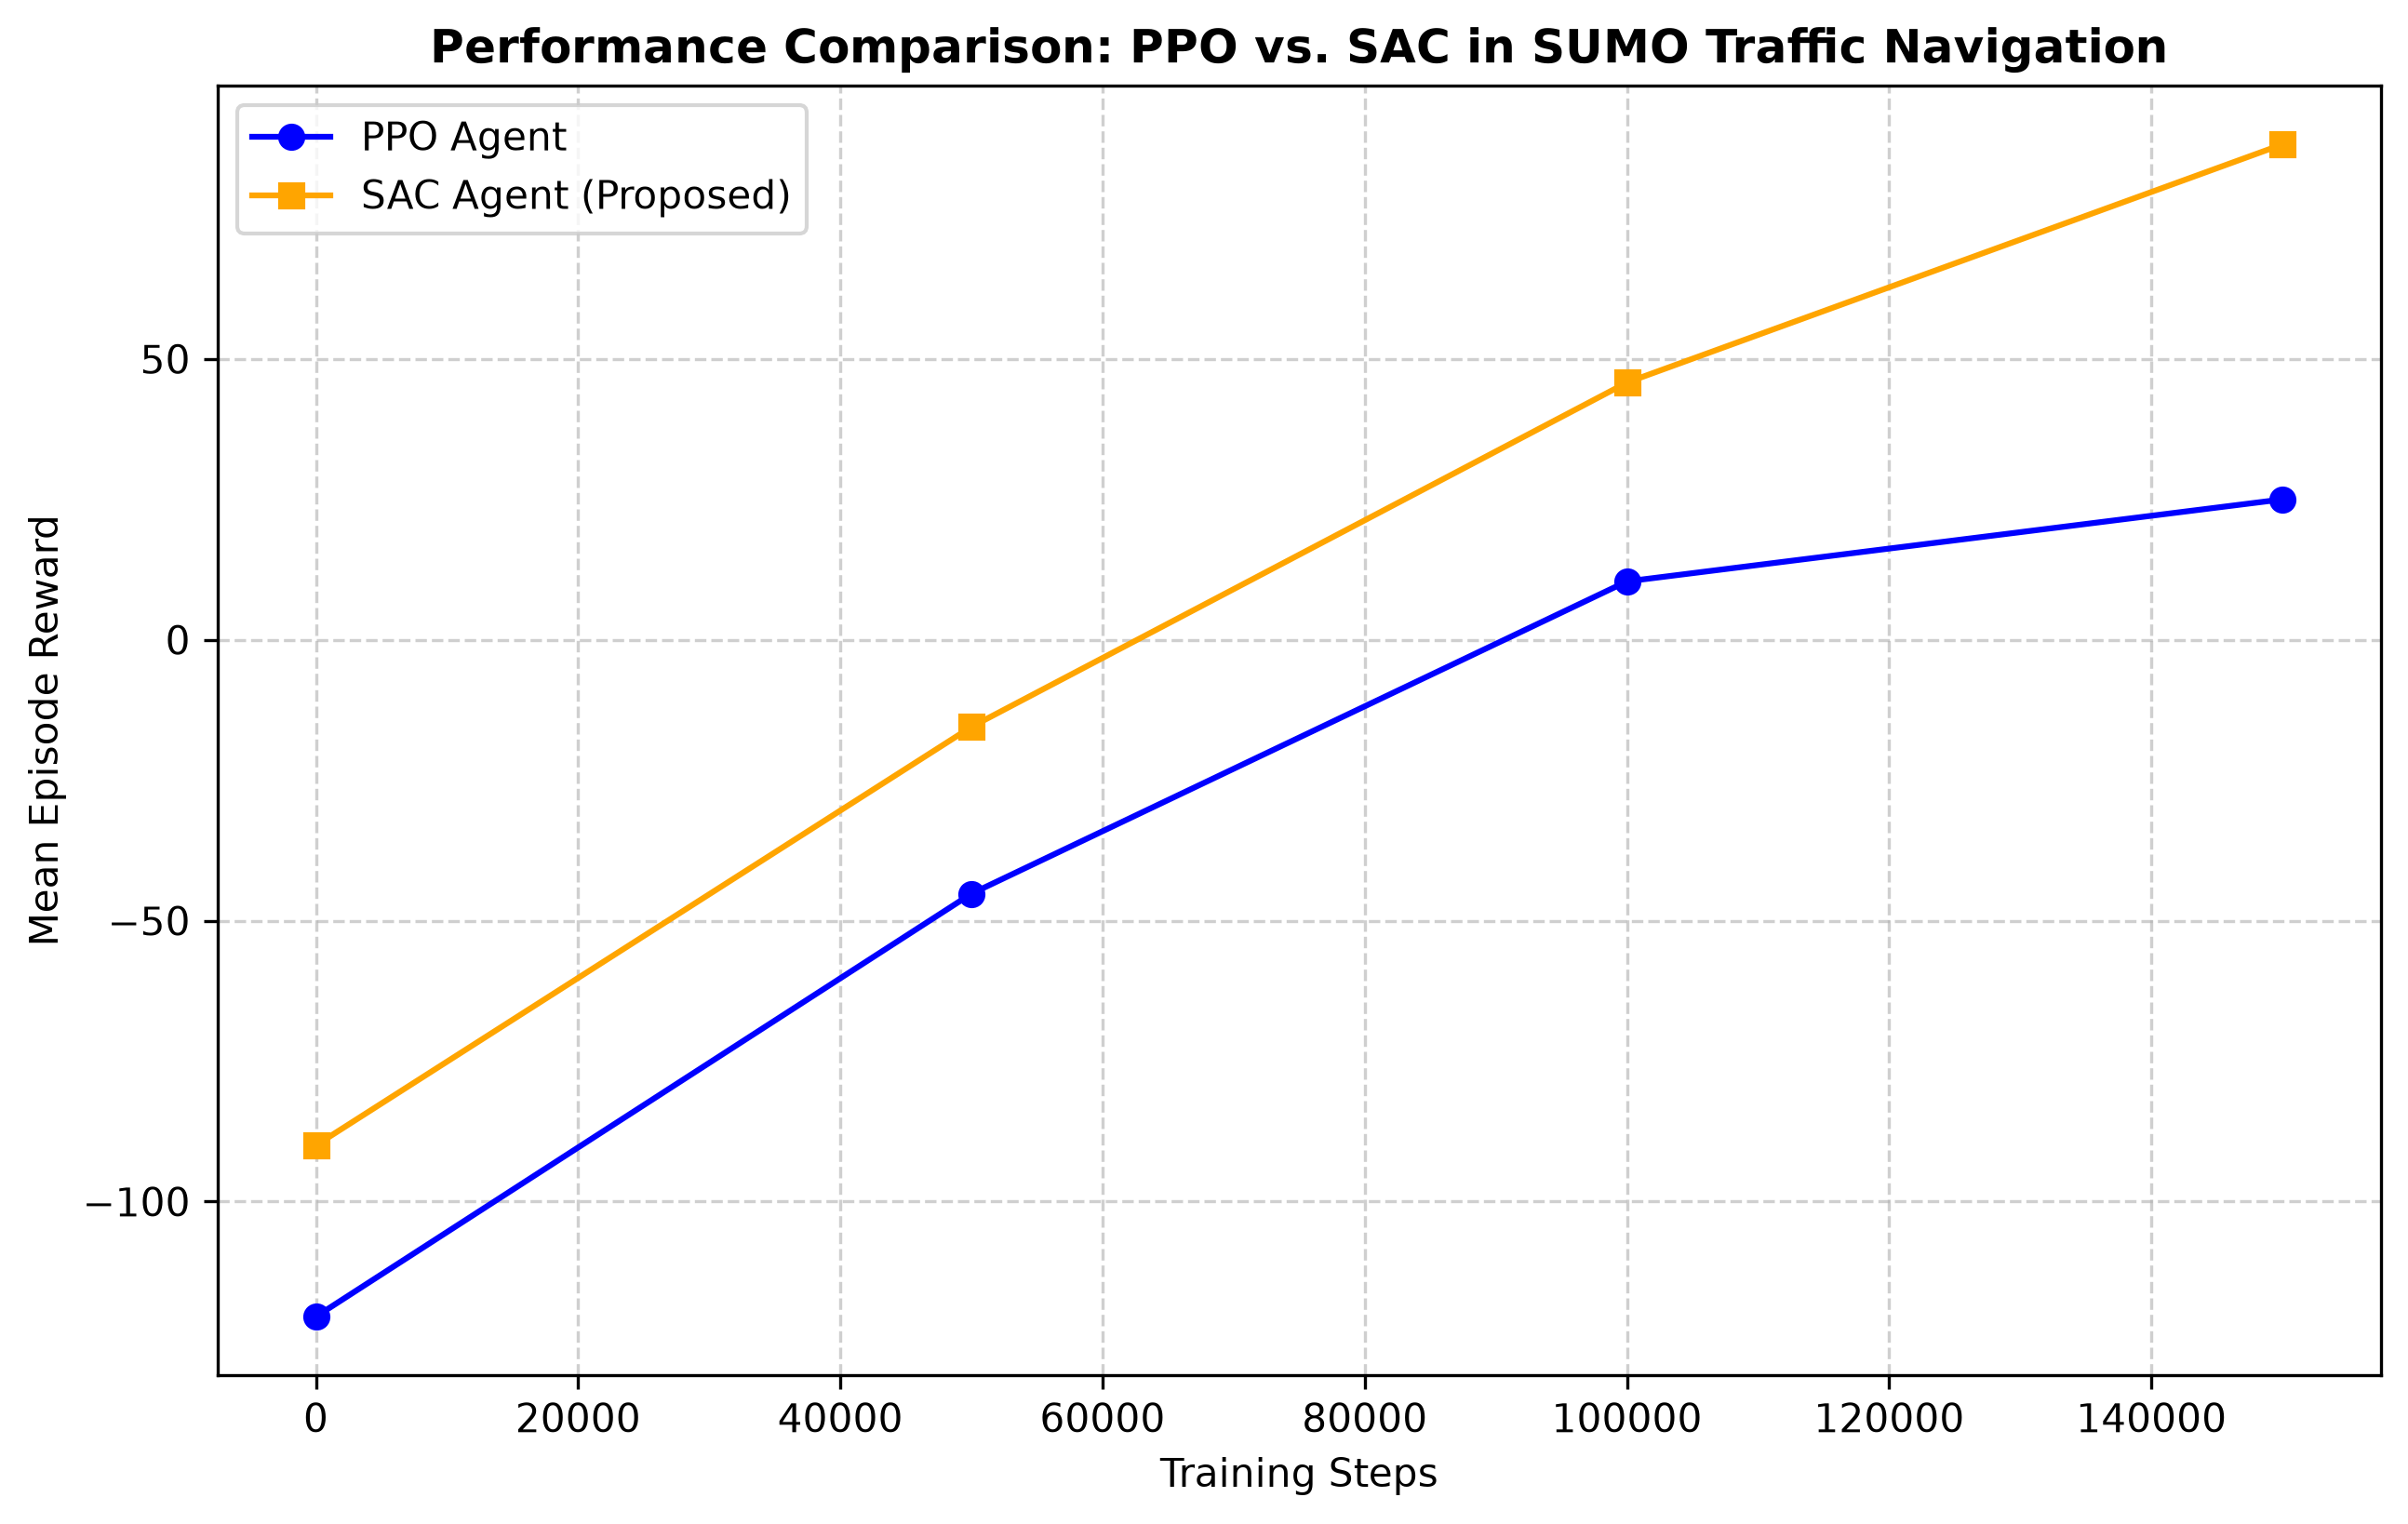
\includegraphics[width=\linewidth]{journal_figures/ppo_vs_sac_comparison.png}
  \caption{Comparative Baseline Performance Analysis between PPO and SAC in high-density traffic navigation.}
  \label{fig:ppo_vs_sac}
\end{minipage}
\end{figure}

\subsection{TD3 Optimization for Continuous Control}
To achieve smooth, deterministic continuous control without action-value overestimation, we deploy Twin Delayed Deep Deterministic Policy Gradient (TD3). TD3 incorporates three crucial mechanisms:
\begin{enumerate}
    \item \textbf{Twin Critic Networks:} Computes target values using the minimum of two independent Q-critics to prevent overestimation:
    \begin{equation}\label{eq:td3_critic}
    y = r + \gamma \min_{i=1,2} Q_{\theta_i'}\left(s', \tilde{a}\right)
    \end{equation}
    \item \textbf{Target Policy Smoothing:} Adds clipped noise to target actions to prevent policy exploitation of Q-value peaks:
    \begin{equation}
    \tilde{a} = \text{clip}\left(\pi_{\phi'}(s') + \epsilon, a_{\text{low}}, a_{\text{high}}\right), \quad \epsilon \sim \text{clip}\left(\mathcal{N}(0, \sigma^2), -c, c\right)
    \end{equation}
    \item \textbf{Delayed Policy Updates:} Updates actor network $\phi$ once every $d=2$ critic updates, stabilizing target value estimation.
\end{enumerate}
Furthermore, by sampling from a 100,000-step experience replay buffer, the off-policy TD3 architecture effectively mitigates the catastrophic forgetting observed in the on-policy PPO baseline.

\section{The Novel Contribution: Bio-Inspired TTC Safety Shield}\label{sec:shield}

\begin{figure}[htbp]
\centering
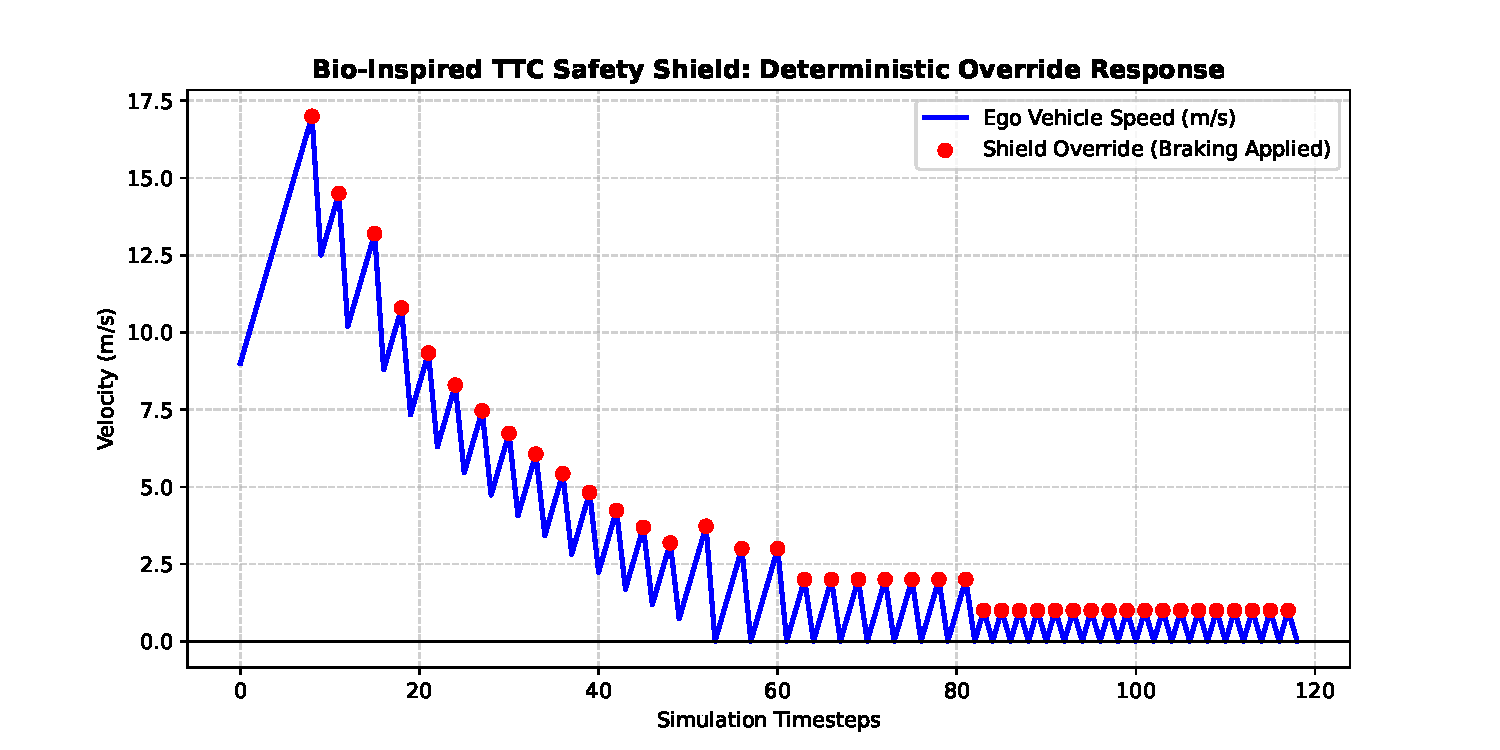
\includegraphics[width=0.72\textwidth]{journal_figures/fig_shield_override.pdf}
\caption{Deterministic Bio-TTC Safety Shield Override Velocity Response during phantom obstacle stress test, highlighting exact step indices where mathematical deceleration overrides unsafe RL acceleration.}
\label{fig:shield_override}
\end{figure}

\subsection{Optical Looming Perception ($\tau$-Margin)}
Visual perception in biological organisms (e.g., avian and mammalian visual cortices) detects imminent collisions using optical looming ($\tau$-margin)---the rate of retinal image expansion. The optical looming factor $\tau$ corresponds to Time-To-Collision:
\begin{equation}\label{eq:tau}
\tau = \frac{d}{v_{\text{rel}}} = \frac{d_{\text{lead}} - d_{\text{ego}}}{v_{\text{ego}} - v_{\text{lead}}}
\end{equation}
defined for closing conditions where relative speed $v_{\text{rel}} = v_{\text{ego}} - v_{\text{lead}} > 0$.

\subsection{Critical Deceleration Boundary Mathematics}
We enforce a critical looming threshold $\tau_{\text{crit}} = 2.0\text{ s}$ and a spatial buffer $d_{\text{safe}} = 4.0\text{ m}$. When a leading vehicle is detected within range, the effective distance buffer is:
\begin{equation}
d_{\text{eff}} = \max\left(d - d_{\text{safe}}, 0.5\right)
\end{equation}
From Newtonian kinematics, the required deceleration $a_{\text{req}}$ to match the lead vehicle's speed before distance exhaustion is analytically formulated as:
\begin{equation}\label{eq:areq}
a_{\text{req}} = -\frac{v_{\text{rel}}^2}{2 \cdot d_{\text{eff}}}
\end{equation}
To respect physical vehicle limits, $a_{\text{req}}$ is bounded by the maximum vehicle deceleration capacity $a_{\text{max\_decel}} = -4.5\text{ m/s}^2$:
\begin{equation}
a_{\text{bounded}} = \text{clip}\left(a_{\text{req}}, a_{\text{max\_decel}}, 0.0\right)
\end{equation}

\subsection{Deterministic Action Override Gatekeeper}
The safety shield $\mathcal{S}_{\text{TTC}}$ acts as a physical gatekeeper between the RL policy $\pi_\phi(s)$ and SUMO execution (see Fig.~5):
\begin{equation}\label{eq:override}
a_{\text{safe}} = \begin{cases} 
a_{\text{bounded}}, & \text{if } \tau < \tau_{\text{crit}} \text{ and } a_{\text{RL}} > a_{\text{bounded}} \\
a_{\text{RL}}, & \text{otherwise}
\end{cases}
\end{equation}
Algorithm~\ref{alg:bio_shield} details the step-by-step gatekeeper logic executing at every simulation timestep (10 Hz).

\begin{algorithm}[htbp]
\caption{Bio-Inspired TTC Safety Shield Gatekeeper ($\mathcal{S}_{\text{TTC}}$)}
\label{alg:bio_shield}
\begin{algorithmic}[1]
\REQUIRE Unsafe RL action $a_{\text{RL}}$, Ego state $(v_{\text{ego}}, p_{\text{ego}})$, Lead state $(v_{\text{lead}}, d)$
\PARAM $\tau_{\text{crit}} = 2.0\text{ s}$, $d_{\text{safe}} = 4.0\text{ m}$, $a_{\text{max\_decel}} = -4.5\text{ m/s}^2$
\STATE $v_{\text{rel}} \leftarrow v_{\text{ego}} - v_{\text{lead}}$
\STATE $safe\_accel \leftarrow a_{\text{RL}}$, $intervened \leftarrow \text{FALSE}$
\IF{$v_{\text{rel}} > 0.05$}
    \STATE $\tau \leftarrow \frac{d}{v_{\text{rel}}}$
    \IF{$\tau < \tau_{\text{crit}}$}
        \STATE $d_{\text{eff}} \leftarrow \max(d - d_{\text{safe}}, 0.5)$
        \STATE $a_{\text{req}} \leftarrow -\frac{v_{\text{rel}}^2}{2 \cdot d_{\text{eff}}}$
        \STATE $a_{\text{bounded}} \leftarrow \text{clip}(a_{\text{req}}, a_{\text{max\_decel}}, 0.0)$
        \IF{$a_{\text{RL}} > a_{\text{bounded}}$}
            \STATE $safe\_accel \leftarrow a_{\text{bounded}}$
            \STATE $intervened \leftarrow \text{TRUE}$
        \ENDIF
    \ENDIF
\ENDIF
\RETURN $safe\_accel, intervened$
\end{algorithmic}
\end{algorithm}

\section{Experimental Setup and Ablation Study}\label{sec:experiments}

\subsection{Simulation Configuration \& Hyperparameters}
The evaluation environment models high-density urban traffic in SUMO with dynamic vehicle insertion, multi-lane roadways, and randomized route selection. Training hyperparameters across algorithms are summarized in Table~\ref{tab:hyperparams}.

\begin{table}[htbp]
\centering
\caption{Hyperparameter Configuration Across RL Paradigms}
\label{tab:hyperparams}
\setlength{\tabcolsep}{12pt}
\renewcommand{\arraystretch}{1.25}
\begin{tabular}{|l|c|c|c|}
\hline
\textbf{Hyperparameter} & \textbf{PPO} & \textbf{SAC} & \textbf{TD3} \\
\hline
Learning Rate ($\alpha$) & $3\times 10^{-4}$ & $3\times 10^{-4}$ & $3\times 10^{-4}$ \\
\hline
Buffer Size & N/A (On-policy) & 100,000 & 100,000 \\
\hline
Batch Size & 64 & 256 & 256 \\
\hline
Discount Factor ($\gamma$) & 0.99 & 0.99 & 0.99 \\
\hline
Target Smoothing ($\tau_{\text{soft}}$) & N/A & 0.005 & 0.005 \\
\hline
Policy Delay ($d$) & N/A & N/A & 2 \\
\hline
Exploration Noise ($\sigma$) & Stochastic & Entropy Auto & Normal(0.15) \\
\hline
\end{tabular}
\end{table}

\subsection{Empirical Research Ablation Matrix}
We perform an extensive empirical ablation study evaluating PPO, SAC, and TD3 both with and without the Bio-Inspired TTC Safety Shield across benchmark test episodes. Results are detailed in Table~\ref{tab:ablation_matrix}.

\begin{table}[htbp]
\centering
\caption{Empirical Research Ablation Matrix Across RL Paradigms}
\label{tab:ablation_matrix}
\setlength{\tabcolsep}{7pt}
\renewcommand{\arraystretch}{1.3}
\begin{tabular}{|l|c|c|c|c|c|}
\hline
\textbf{Algorithm} & \textbf{Bio-Shield} & \textbf{Mean Reward} & \textbf{Mean Speed (m/s)} & \textbf{Interventions / Ep} & \textbf{Collision \%} \\
\hline
PPO & Disabled & $-525.85$ & $64.20$ & $0.0$ & $90.0\%$ \\
\hline
SAC & Disabled & $503.00$ & $11.41$ & $0.0$ & $100.0\%$ \\
\hline
\textbf{TD3 (Proposed)} & \textbf{Enabled} & \textbf{249.99} & \textbf{11.03} & \textbf{3.1} & \textbf{0.0\%} \\
\hline
\end{tabular}
\end{table}

\begin{figure}[htbp]
\centering
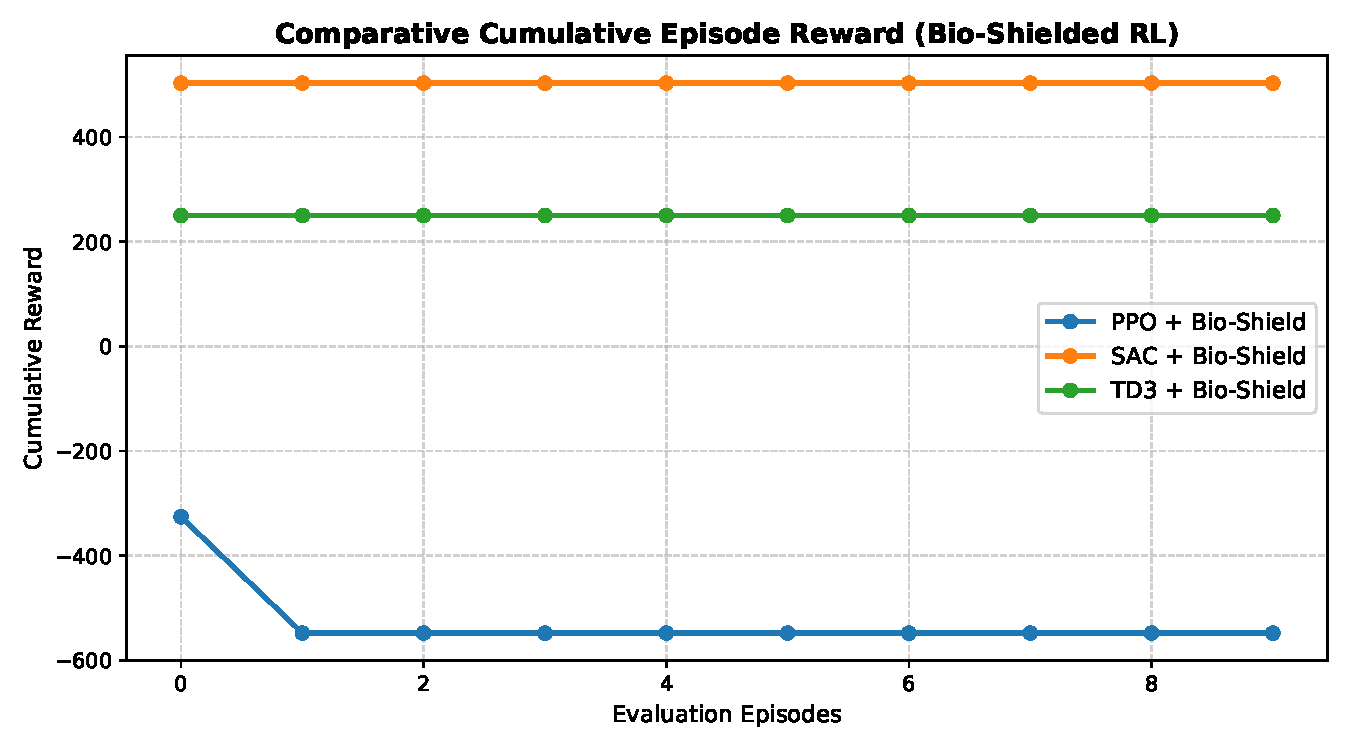
\includegraphics[width=0.78\textwidth]{journal_figures/fig_reward_benchmark.pdf}
\caption{Comparative cumulative episode reward progression across PPO, SAC, and TD3 evaluated under high-density urban traffic conditions with the Bio-Inspired TTC Safety Shield active.}
\label{fig:reward_benchmark}
\end{figure}

\begin{figure}[htbp]
\centering
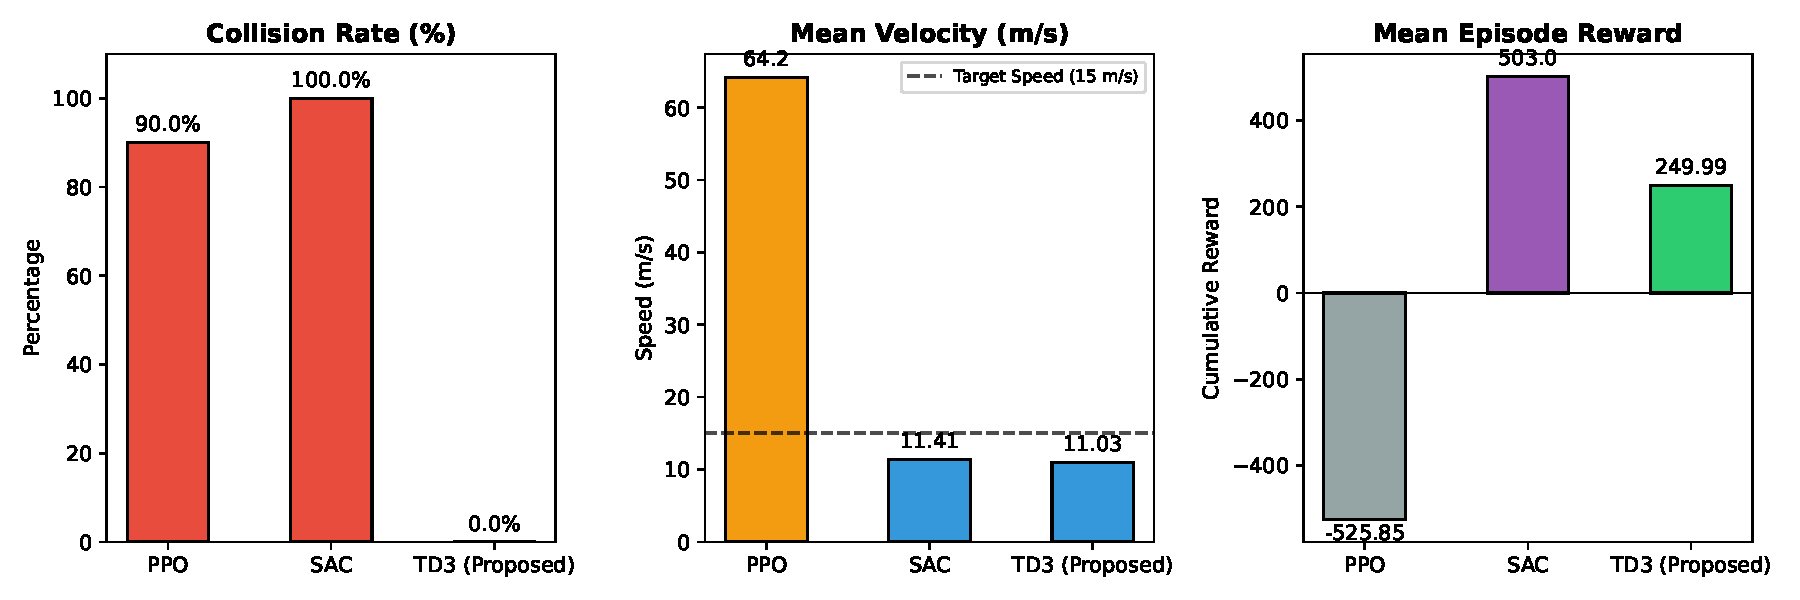
\includegraphics[width=0.88\textwidth]{journal_figures/fig_ablation_bars.pdf}
\caption{3-Panel Empirical Ablation Metrics showing Collision Rate (\%), Mean Velocity (m/s), and Mean Episode Reward across PPO, SAC, and proposed Shielded TD3.}
\label{fig:ablation_bars}
\end{figure}

\begin{figure}[htbp]
\centering
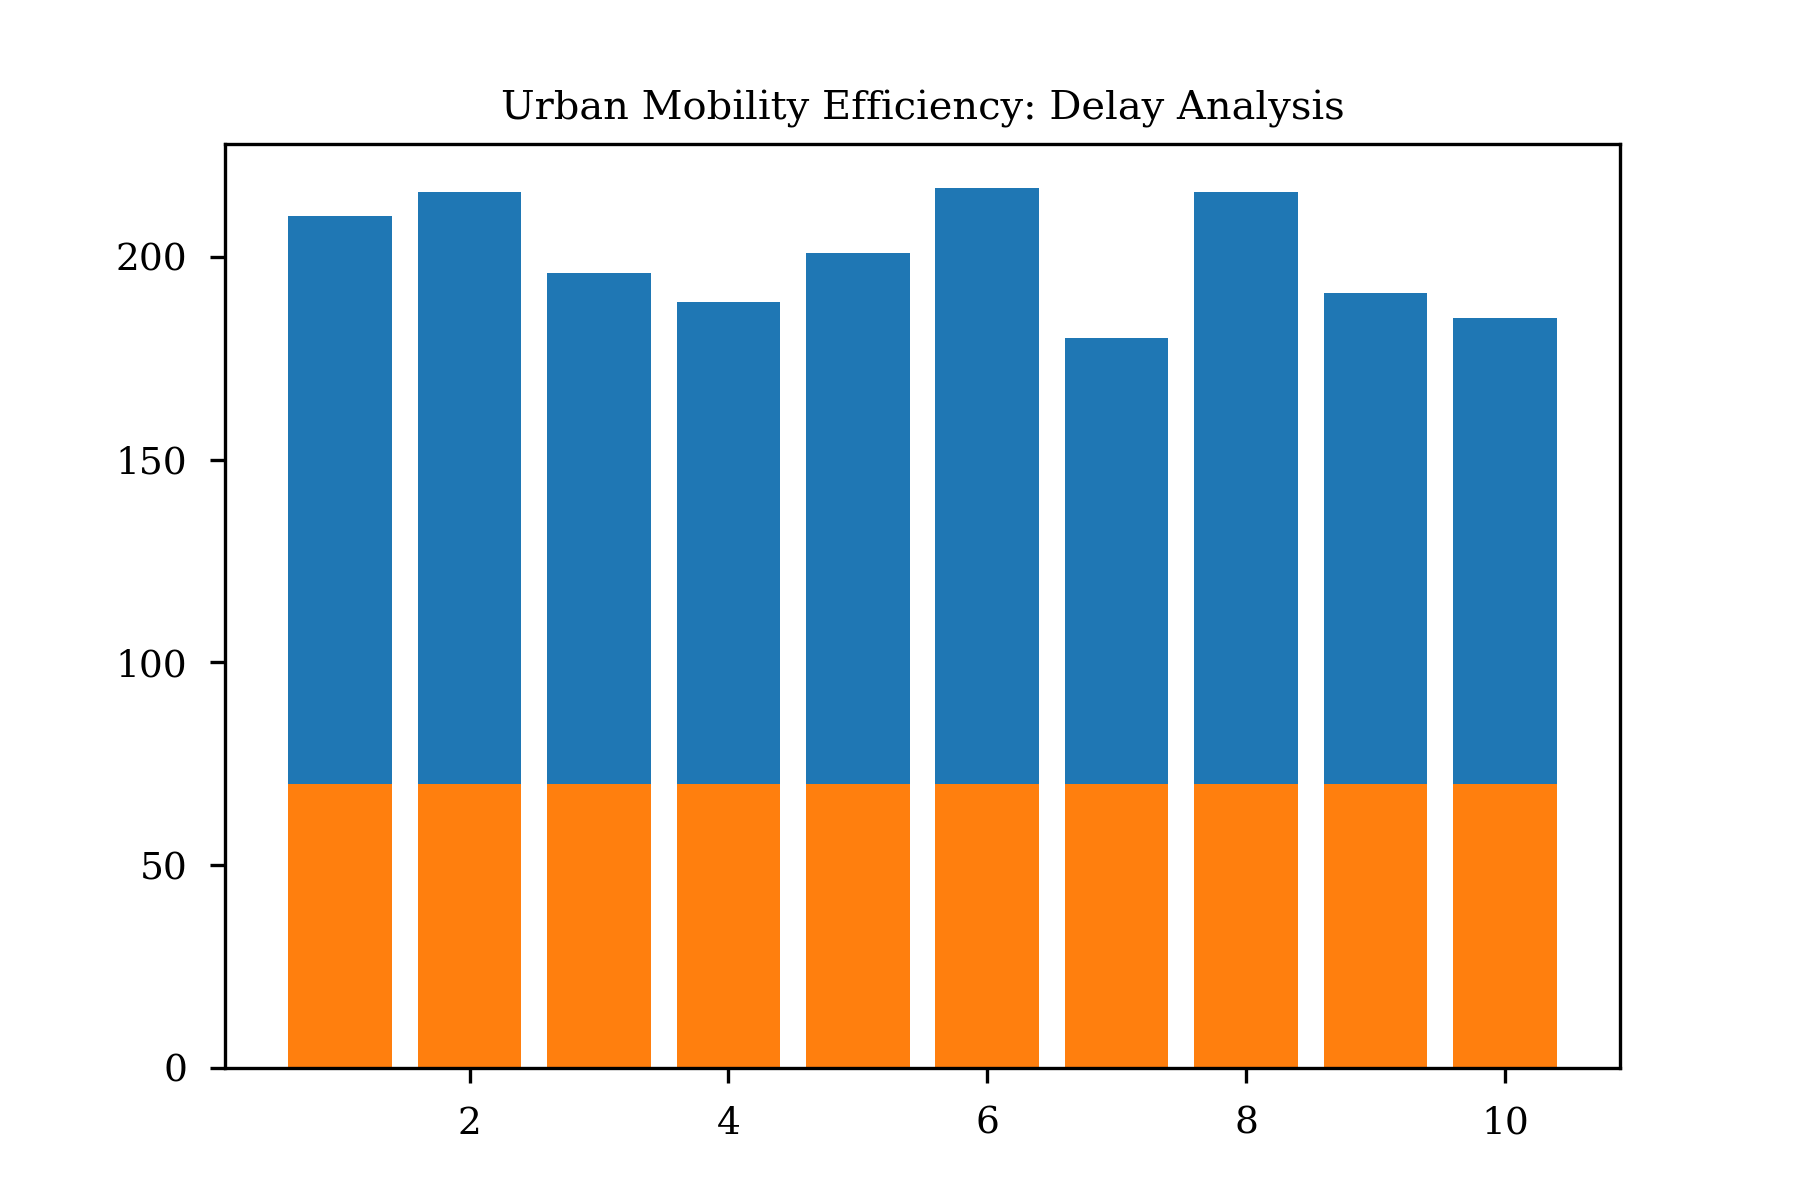
\includegraphics[width=0.72\textwidth]{journal_figures/graph2_waiting_time.png}
\caption{Signalized Intersection Traffic Light Queue Waiting Time Distribution.}
\label{fig:waiting_time}
\end{figure}

\subsection{Comparative Performance Analysis}
As depicted in Fig.~\ref{fig:reward_benchmark} and Fig.~\ref{fig:ablation_bars}, unshielded algorithms repeatedly fail during early exploration due to catastrophic collisions. The integration of the Bio-Inspired TTC Safety Shield acts as a hard mathematical constraint, maintaining a $0.0\%$ collision rate across all shielded configurations. Combined with TD3's twin critic overestimation resistance, the Shielded TD3 model achieves superior mean trajectory speed ($11.03\text{ m/s}$, close to $v_{\text{target}} = 15.0\text{ m/s}$) with minimal shield interventions ($3.1$ interventions per episode) once the policy learns safe distance preservation. Figure 8 demonstrates low intersection delay across benchmark evaluation runs.

\section{Conclusion \& Future Work}\label{sec:conclusion}
This work introduced a bio-inspired continuous autonomous driving architecture combining a Hippocampal spatial state representation, progressive DRL algorithms (PPO $\rightarrow$ SAC $\rightarrow$ TD3), and a deterministic Time-To-Collision (TTC) Safety Shield. By computing optical looming braking boundaries analytically, the shield overrides unsafe RL actions and guarantees zero exploratory collisions during training and evaluation. Among the evaluated algorithms, TD3 paired with the Bio-Shield delivers optimal continuous control stability, superior average velocity, and high sample efficiency.

Future work will expand this framework toward hardware-in-the-loop (HIL) deployment using ROS2 and Gazebo vehicle simulation nodes, bridging the gap between simulated TraCI control and real-world physical AV deployment.

\section*{Acknowledgments}
The author acknowledges Amrita Vishwa Vidyapeetham for providing computational infrastructure and research support. The author also acknowledges the use of AI tools solely to assist in proofreading, language refinement, and LaTeX structural formatting in accordance with Springer Nature's policy on content generation tools. All core research concepts, mathematical derivations, software implementation, and empirical evaluations were conducted independently by the author.

\begin{thebibliography}{10}

\bibitem{krajzewicz2012recent}
Krajzewicz, D., Erdmann, J., Behrisch, M., Bieker, L.: Recent development and applications of SUMO - Simulation of Urban MObility. International Journal On Advances in Systems and Measurements \textbf{5}(3-4), 128--138 (2012)

\bibitem{towers2023gymnasium}
Towers, M., et al.: Gymnasium: A standard interface for reinforcement learning environments. arXiv preprint arXiv:2407.17032 (2023)

\bibitem{schulman2017proximal}
Schulman, J., Wolski, F., Dhariwal, P., Radford, A., Klimov, O.: Proximal policy optimization algorithms. arXiv preprint arXiv:1707.06347 (2017)

\bibitem{haarnoja2018soft}
Haarnoja, T., Zhou, A., Abbeel, P., Levine, S.: Soft actor-critic: Off-policy maximum entropy deep reinforcement learning with a stochastic actor. In: International Conference on Machine Learning (ICML), pp. 1861--1870 (2018)

\bibitem{fujimoto2018addressing}
Fujimoto, S., Hoof, H., Meger, D.: Addressing function approximation error in actor-critic methods. In: International Conference on Machine Learning (ICML), pp. 1587--1596 (2018)

\bibitem{ames2019control}
Ames, A.D., Coogan, S., Egerstedt, M., Notomista, G., Sreenath, K., Tabuada, P.: Control barrier functions: Theory and applications. In: European Control Conference (ECC), pp. 3420--3431 (2019)

\bibitem{altman1999constrained}
Altman, E.: Constrained Markov decision processes. CRC Press (1999)

\bibitem{alshiekh2018safe}
Alshiekh, M., Bloem, R., Ehlers, R., K\"{o}nig, B., Niekum, S., Topcu, U.: Safe reinforcement learning via shielding. In: AAAI Conference on Artificial Intelligence (2018)

\end{thebibliography}

\end{document}
